\documentclass[11pt,a4paper]{article}
\usepackage[T1]{fontenc}
\usepackage[utf8]{inputenc}
\usepackage{lmodern,microtype}
\usepackage{amsmath,amssymb,amsthm,mathtools,bm}
\usepackage{booktabs,array,tabularx,longtable}
\usepackage{graphicx,float,caption}
\usepackage{xcolor}
\usepackage[margin=20mm]{geometry}
\usepackage{enumitem}
\usepackage{fancyhdr}
\usepackage[hidelinks]{hyperref}
\hypersetup{
  pdftitle={FIN ST70--ST81: Independent Replay, Spin Covers, and Conditional Source Architecture},
  pdfauthor={Krzysztof Żuchowski},
  pdfsubject={Analytical and computational execution of FIN programs ST70--ST81},
  pdfkeywords={FIN, rational replay, feedback, central extension, spin cover, refinement, CPTP, thermodynamics, pseudo-arclength, chirality}
}
\setlength{\parindent}{0pt}
\setlength{\parskip}{0.50em}
\setlength{\emergencystretch}{2em}
\setlength{\headheight}{14pt}
\setlist[itemize]{leftmargin=1.55em,itemsep=0.16em,topsep=0.2em}
\setlist[enumerate]{leftmargin=1.75em,itemsep=0.16em,topsep=0.2em}
\pagestyle{fancy}
\fancyhf{}
\lhead{FIN ST70--ST81}
\rhead{Release 10.60}
\cfoot{\thepage}
\newtheorem{theorem}{Theorem}[section]
\newtheorem{proposition}[theorem]{Proposition}
\newtheorem{corollary}[theorem]{Corollary}
\newcommand{\proven}{\textcolor{green!40!black}{\textbf{[PROVEN]}}}
\newcommand{\strong}{\textcolor{blue!70!black}{\textbf{[STRONG EVIDENCE]}}}
\newcommand{\conditional}{\textcolor{black!60}{\textbf{[CONDITIONAL]}}}
\newcommand{\constructed}{\textcolor{violet!70!black}{\textbf{[CONSTRUCTED]}}}
\newcommand{\failed}{\textcolor{red!72!black}{\textbf{[REFUTED IN CLASS]}}}
\newcommand{\statusboundary}{\textcolor{orange!80!black}{\textbf{[BOUNDARY]}}}
\newcommand{\resultbox}[1]{\begin{center}\fcolorbox{blue!60!black}{blue!4}{\parbox{0.92\textwidth}{#1}}\end{center}}

\begin{document}

\pagenumbering{gobble}
\begin{titlepage}
\centering
\vspace*{1.15cm}
{\LARGE\bfseries FIN ST70--ST81\par}
\vspace{0.35cm}
{\Large Independent Replay, Spin Covers, and Conditional Source Architecture\par}
\vspace{0.40cm}
{\large Exact certificate audit, time-oriented feedback, central extensions, fine-data refinement, robust counts, CPTP cones, thermodynamic resources, fold continuation, backreaction, chirality, and signed custody\par}
\vspace{1.00cm}
{\Large Krzysztof Żuchowski\par}
\vspace{0.24cm}
{\large Independent Researcher --- Fractal Information Theory Project\par}
{\large ORCID: 0009-0002-0909-3613\par}
\vspace{0.80cm}
{\large FIN Release 10.60 --- Version 1.0.0\par}
{\large August 11, 2026\par}
\vfill
\begin{minipage}{0.89\textwidth}
\textbf{Scope.} This report executes ST70--ST81. It independently audits the exported ST58 proof inequalities, classifies the extra order required for positive gain, constructs and obstructs a spin cover, replaces stationary refinement by a fine-record code, strengthens the synthetic receiver, classifies the complete CPTP intertwiner cone, tests thermodynamic-resource minimality, crosses the ST65 fold, and updates the physical-source architecture.\par
\textbf{Method.} Exact rational arithmetic, finite group cohomology over $\mathbb F_2$, finite-dimensional operator theory, convex rate--distortion analysis, robust information bounds, Choi constraints, removal countermodels, pseudo-arclength continuation, bifurcation analysis, Ed25519 verification, and twenty-four live tests.\par
\textbf{Epistemic rule.} An exact replay of exported inequalities is not an independent regeneration of their upstream transcendental enclosures. A numerical fold with a tiny residual is not an interval theorem. A constructed cover, response cone, fine-data code, or signature protocol is not a strict physical source.\par
\textbf{Repository snapshot.} Git commit \texttt{d6a38efbb05dfb472e2dc21b546fa793317d4fb8}; additional local artifacts are recorded by the release manifest.\par
\textbf{Repository.} \url{https://github.com/hyconiek/Fractal-Nadsoliton-Theory}\par
\textbf{License.} CC BY 4.0.
\end{minipage}
\end{titlepage}
\pagenumbering{arabic}

\begin{abstract}
This report completes twelve local programs. ST70 replays every decisive serialized ST58 acceptance inequality using only exact standard-library rational arithmetic. The collision polynomial has a strictly positive interval at the left endpoint, a strictly negative interval at the right endpoint, and derivative
\[
-0.530298440331365 < p'(s) < -0.530298440318102.
\]
The root is therefore unique in the exported bracket. The replay is independent of the ST58 implementation but does not regenerate the upstream cosine, Fourier, inverse, or Krawczyk enclosures.

ST71 proves that on the five-dimensional reflection-odd sector uniform gradient-flow gain at rate $\mu$ is equivalent to the one-sided response condition $H_-\preceq-\mu I$. This condition evades the ST59 sign flip precisely because it is an added time/order orientation. ST72 constructs the nontrivial central extension $C_{24}\to C_{12}$ using the carry cocycle
\[
c(a,b)=\left\lfloor\frac{a+b}{12}\right\rfloor\pmod2.
\]
All 1,728 cocycle equations pass, while the coboundary system has rank 10 and augmented rank 11. The spin cover exists, but scalar strict data see only the $C_{12}$ quotient and cannot select between $C_{12}\times\mathbb Z_2$ and $C_{24}$.

ST73 proves that supplied fine-only data and a rate penalty uniquely select a dyadic lift, while every lift can be selected by a suitable extra record; no canonical refinement follows from coarse $A$. ST74 adds declared loss, dark-count, and calibration uncertainty. The conservative synthetic bracket becomes 32 necessary versus 14,301 sufficient total uniformly sampled joint events, corresponding to expected means of 3 and 1,192 events per preparation. These are not laboratory counts.

ST75 completely characterizes the CPTP intertwiners between strict unitary evolution and $A$-dephasing. Every intertwiner factors through the 22-dimensional equal-energy block algebra; the full complex linear space has dimension $22^2=484$, and its CPTP members are exactly the Choi-positive trace-preserving maps in that space. ST76 proves relative independent necessity of four thermodynamic resource types: an energy scale, an entropy unit, a Gibbs reference/bath, and a Gibbs-preserving process with operational heat/work semantics.

ST77 numerically crosses the previously unresolved localized fold. It identifies a simple fold at
\[
\kappa_{\rm fold}=0.01658905238638291,
\qquad \operatorname{IPR}=0.9776497495,
\]
with augmented-system residual $8.33\times10^{-17}$ and then follows a return branch. This corrects ``termination'' to ``fold'' but is not interval-certified and does not reach strict coupling. ST78 proves that coupling the constructed ST66 order parameter to the strict first doublet quenches its twelve nonzero branches at
\[
g_c=\mu/\lambda_1=0.4641164063;
\]
unit coupling lies above this threshold. ST79 proves a reflection-stabilizer no-go for deterministic strict-sourced Bargmann chirality. ST80 exports a signed validator with synthetic Ed25519 fixtures. ST81 retains all nine strict physical-source groups. The mathematical architecture is sharper; no new physical-source closure follows.
\end{abstract}

\textbf{Status vocabulary.} \proven{} denotes an exact finite or analytic result in the declared class. \strong{} denotes robust numerical evidence without interval/global proof. \conditional{} denotes a theorem after explicit additional premises. \constructed{} denotes a complete object or protocol whose strict source is absent. \failed{} denotes a destroyed implication in its declared class. \statusboundary{} records a precise non-implication.

\tableofcontents
\newpage

\section{Frozen object and research discipline}

The strict finite working operator remains
\begin{equation}
W_{xx}=0,\qquad
W_{xy}=\frac{\cos(0.18575d(x,y)+0.16250)}{1+d(x,y)^{1.8}}\quad(x\ne y),
\qquad A=sI-W,
\label{eq:strict}
\end{equation}
on $C_{12}$, with $s=1.660307278766099$ to the displayed precision. Thus
\[
\langle f,Af\rangle=\frac12\sum_{x,y}W_{xy}|f_x-f_y|^2\ge0.
\]
The zero diagonal is part of the definition. The legacy ontological kernel remains an intermediate bridge object. This batch neither substitutes it for~\eqref{eq:strict}, completes its strict continuation, nor transfers any legacy physical role.

The questions are:
\begin{enumerate}
\item Which part of the ST58 certificate survives an independent arithmetic implementation?
\item What extra mathematical order is necessary and sufficient for positive adaptive gain?
\item Does strict cyclic symmetry carry a canonical spin/projective lift?
\item Can fine data remove refinement nonuniqueness without smuggling in a selector?
\item What are the full operational intertwiners and minimal thermodynamic conversion resources?
\item Was the localized ST65 branch terminated, folded, or continued?
\item Can strict doublet backreaction or a Bargmann invariant create orientation?
\item Can executable custody syntax be strengthened without confusing signatures with real independence?
\end{enumerate}

\resultbox{\textbf{Principal conclusion.} The batch separates three layers sharply. Exact finite mathematics supplies a nontrivial $C_{24}$ cover, a complete CPTP cone, gain and chirality obstructions, and a conditional backreaction threshold. Numerical continuation reveals that ST65 encountered a fold rather than termination. None of these results selects the cover, response orientation, fine record, dimensional scale, physical process, or experimental carrier from strict $A$.}

\section{Outcome matrix}

\small
\begin{longtable}{@{}p{0.055\textwidth}p{0.30\textwidth}p{0.23\textwidth}p{0.32\textwidth}@{}}
\toprule
ID & Object & Outcome & Exact boundary\\
\midrule
\endfirsthead
\toprule
ID & Object & Outcome & Exact boundary\\
\midrule
\endhead
ST70 & Exact-rational ST58 replay & \proven{} partial independent audit & Upstream transcendental enclosures retained\\
ST71 & Time-oriented response cone & \proven{} relative classification & Curvature sign/order is added\\
ST72 & $C_{24}$ spin cover & \proven{} construction and no-source & Strict scalar quotient does not choose lift\\
ST73 & Fine-data rate--distortion refinement & \conditional{} & Fine record and penalty added\\
ST74 & Nuisance-robust count bracket & \proven{} for synthetic sets & Not calibrated apparatus performance\\
ST75 & Complete CPTP intertwiner cone & \proven{} & Dephasing, not vertex heat\\
ST76 & Thermodynamic-resource minimality & \proven{} relative & Conversion resources remain external\\
ST77 & Pseudo-arclength fold & \strong{} & No interval certificate or $\kappa=1$ link\\
ST78 & Strict-doublet backreaction threshold & \proven{} conditional & Potential and coupling inserted\\
ST79 & Bargmann chirality source & \failed{} in stabilizer class & State/boundary breaking remains possible\\
ST80 & Signed custody validator & \constructed{} & Test keys do not create identity/custody\\
ST81 & Source architecture & \proven{} relative no-reduction & Nine source groups retained\\
\bottomrule
\end{longtable}
\normalsize

\section{ST70 --- Exact-rational replay of the collision certificate}

The ST58 root was obtained after setting $x=1/s$ in
\[
a x^2+b x+c=0.
\]
Equivalently, the speed satisfies
\[
p(s)=a+bs+cs^2=0.
\]
ST70 parses every serialized decimal interval as an exact rational number. It neither imports the ST58 interval functions nor invokes \texttt{mpmath}. Exact interval multiplication gives
\begin{align*}
p(s_{\rm L})&\subset[1.0584003887317,6.3246958807246]\times10^{-12},\\
p(s_{\rm R})&\subset[-6.3246266168889,-1.0583311248089]\times10^{-12},\\
p'([s_{\rm L},s_{\rm R}])&\subset[-0.530298440331365,-0.530298440318102].
\end{align*}
It also exactly checks positivity of all pole, residue, nonlinear-inclusion, and linear-inclusion margins and verifies that all comparison radii and the nonlinear defect are below one.

\begin{theorem}[Exported-bracket uniqueness]
Conditional on the correctness of the interval quantities serialized by ST58, the collision polynomial has exactly one zero in
\[
1.278014751813487\le s_*\le1.2780147518274094.
\]
\end{theorem}

\statusboundary{} This is a genuinely independent acceptance-inequality replay. It is not an independent reconstruction of trigonometric weights, Fourier intervals, the stationary box, or matrix preconditioner errors. ST82 must regenerate those upstream objects using Arb, Sage, Lean, or another independently specified directed-arithmetic stack.

\begin{figure}[H]
\centering
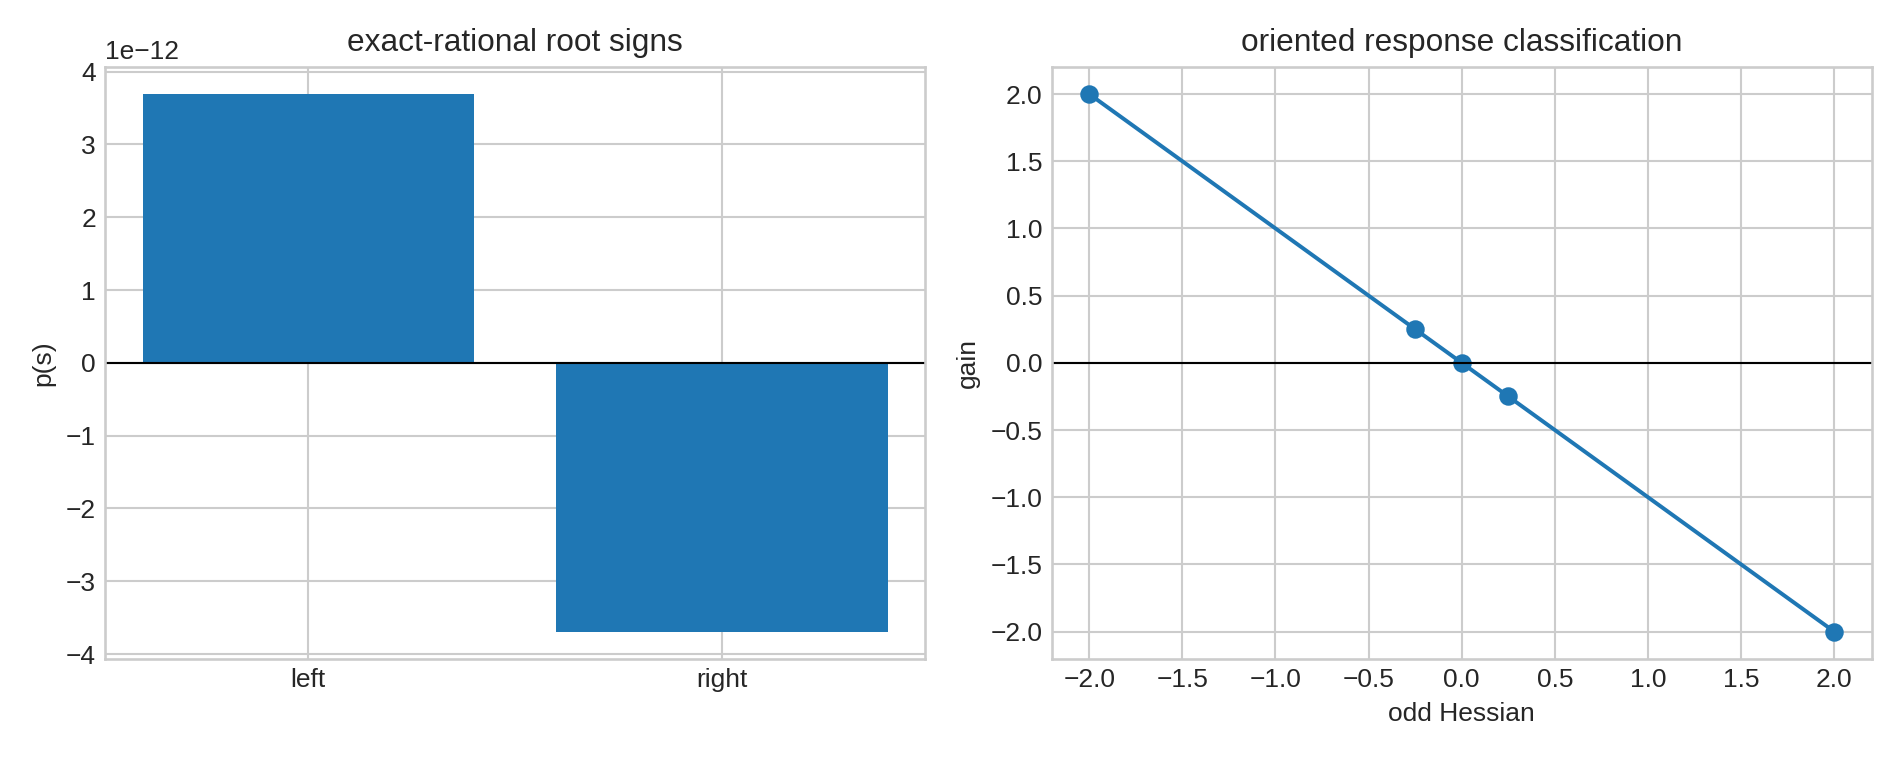
\includegraphics[width=0.94\textwidth]{FIN_ST70_ST81_Figures/st70_replay_st71_gain.png}
\caption{ST70 exact endpoint signs and ST71 gain/curvature equivalence.}
\end{figure}

\section{ST71 --- What positive feedback mathematically requires}

Reflection on $C_{12}$ has a five-dimensional odd state subspace, spanned by
\[
e_j^-=(e_j-e_{-j})/\sqrt2,\qquad j=1,\ldots,5.
\]
Let $H_-$ be the Hessian of an adaptive response functional on that subspace. The linearized Euclidean gradient law is
\[
\dot\xi=-H_-\xi.
\]

\begin{theorem}[Oriented gain cone]
Uniform amplification at rate at least $\mu>0$ for every reflection-odd perturbation is equivalent to
\[
H_-\preceq-\mu I.
\]
If this one-sided order is removed and the response class is closed under $H_-\mapsto-H_-$, positive and negative gains coexist with the same strict operator and stationary symmetry data.
\end{theorem}

This answers the positive-feedback question narrowly but decisively. Symmetry supplies the response sector; it does not supply the arrow that declares negative response curvature physically admissible and the opposite sign inadmissible. A time orientation, entropy-production order, passivity convention, or causal response law must pay that sign.

\statusboundary{} The theorem identifies a necessary and sufficient premise in a declared linear response class. It does not derive that premise, its magnitude $\mu$, or a physical clock from FIN.

\section{ST72 --- A spin cover exists, but strict data do not choose it}

Represent elements of $C_{12}$ by $0,\dots,11$ and define
\[
c(a,b)=\left\lfloor\frac{a+b}{12}\right\rfloor\pmod2.
\]
The code evaluates all $12^3=1{,}728$ equations
\[
c(a,b)+c(a+b,d)=c(b,d)+c(a,b+d)\pmod2
\]
and finds zero defects. The normalized coboundary system $c=\delta f$ has coefficient rank 10 and augmented rank 11, proving inconsistency.

\begin{theorem}[Two cyclic central lifts]
The central $\mathbb Z_2$ lift of a generator $g\in C_{12}$ has an invariant sign $\widetilde g^{12}=\pm1$. Since 12 is even, replacing $\widetilde g$ by $-\widetilde g$ cannot change it. The $+1$ class gives $C_{12}\times\mathbb Z_2$; the carry cocycle realizes the nontrivial $-1$ class $C_{24}$. Both project to the same scalar $C_{12}$ action.
\end{theorem}

The strict operator commutes with the base rotation to residual $6.3\times10^{-16}$. Every scalar construction from $A$ therefore factors through the quotient and is blind to the central sign.

\statusboundary{} ST72 constructs the representation type needed by the half-angle texture, but simultaneously proves that scalar strict data do not select it. $C_{24}$ is an admissible sector axiom, not a QW-2191 solution.

\begin{figure}[H]
\centering
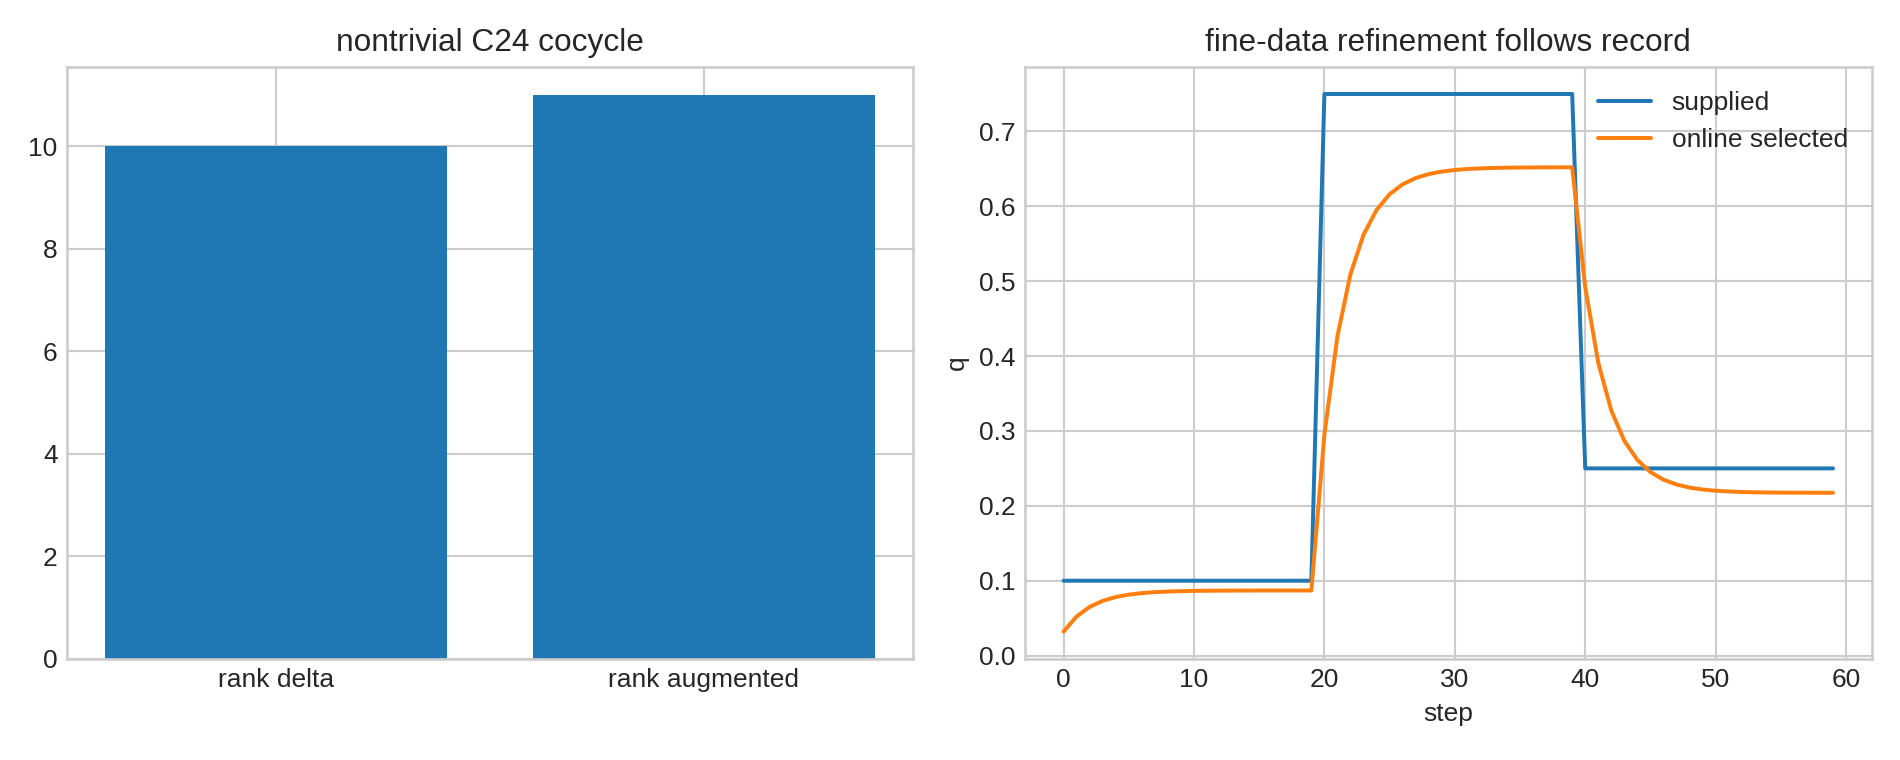
\includegraphics[width=0.94\textwidth]{FIN_ST70_ST81_Figures/st72_spin_st73_refinement.png}
\caption{The nontrivial cocycle is not a coboundary; a nonstationary lift follows the supplied fine record.}
\end{figure}

\section{ST73 --- Nonstationary fine-data refinement}

For the dyadic family $A_{24}(q)$, let $F_-$ embed the 12-dimensional fine-only subspace $(v,-v)/\sqrt2$. Its trace statistic is affine:
\[
y(q)=\frac1{12}\operatorname{tr}(F_-^*A_{24}(q)F_-)-y(0)=2q.
\]
Given an observed fine statistic $y$ and rate penalty $\lambda>0$, define
\[
\mathcal D(q)=\frac12(gq-y)^2+\frac\lambda2q^2,qquad q\ge0,qquad g=2.
\]

\begin{theorem}[Conditional refinement selector]
$\mathcal D$ is strictly convex and has the unique minimizer
\[
q_* = \max\left(0,\frac{gy}{g^2+\lambda}\right).
\]
Conversely, every $q_0\ge0$ is the unique minimizer for $y=(g^2+\lambda)q_0/g$.
\end{theorem}

Thus a fine record can remove ST18/ST30 nonuniqueness, and an online gradient law can adapt to a nonstationary record. The converse shows why this does not derive a canonical fractal refinement: the supplied fine statistic and complexity penalty carry the choice.

\statusboundary{} No strict compression process, rate functional, fine observation, or universality theorem is obtained.

\section{ST74 --- Robust synthetic count design}

The frozen ST51 joint distributions are mixed independently with a uniform loss/dark component $\epsilon\in[0,0.12]$. Each hypothesis is also enlarged by a total-variation calibration ball of radius $0.003$. A $241\times241$ nuisance grid gives the closest mixture at $\epsilon_P=\epsilon_Q=0.12$ with pre-calibration $L^1$ separation $0.2536926361$. Paying both TV balls leaves
\[
\Delta_{1,\rm robust}=0.2416926361.
\]

For a 144-symbol joint experiment, KL data processing supplies a necessary count of 32 total events for both idealized errors to be at most 0.01. The distribution-free multinomial bound
\[
\Pr(\|\widehat P-P\|_1\ge\Delta/2)
\le 2^{144}\exp(-n\Delta^2/8)
\]
gives the conservative sufficient count 14,301. With preparations chosen uniformly at random, these correspond to expected means of 3 and 1,192 events per preparation. They are not fixed-stratum guarantees.

\begin{figure}[H]
\centering
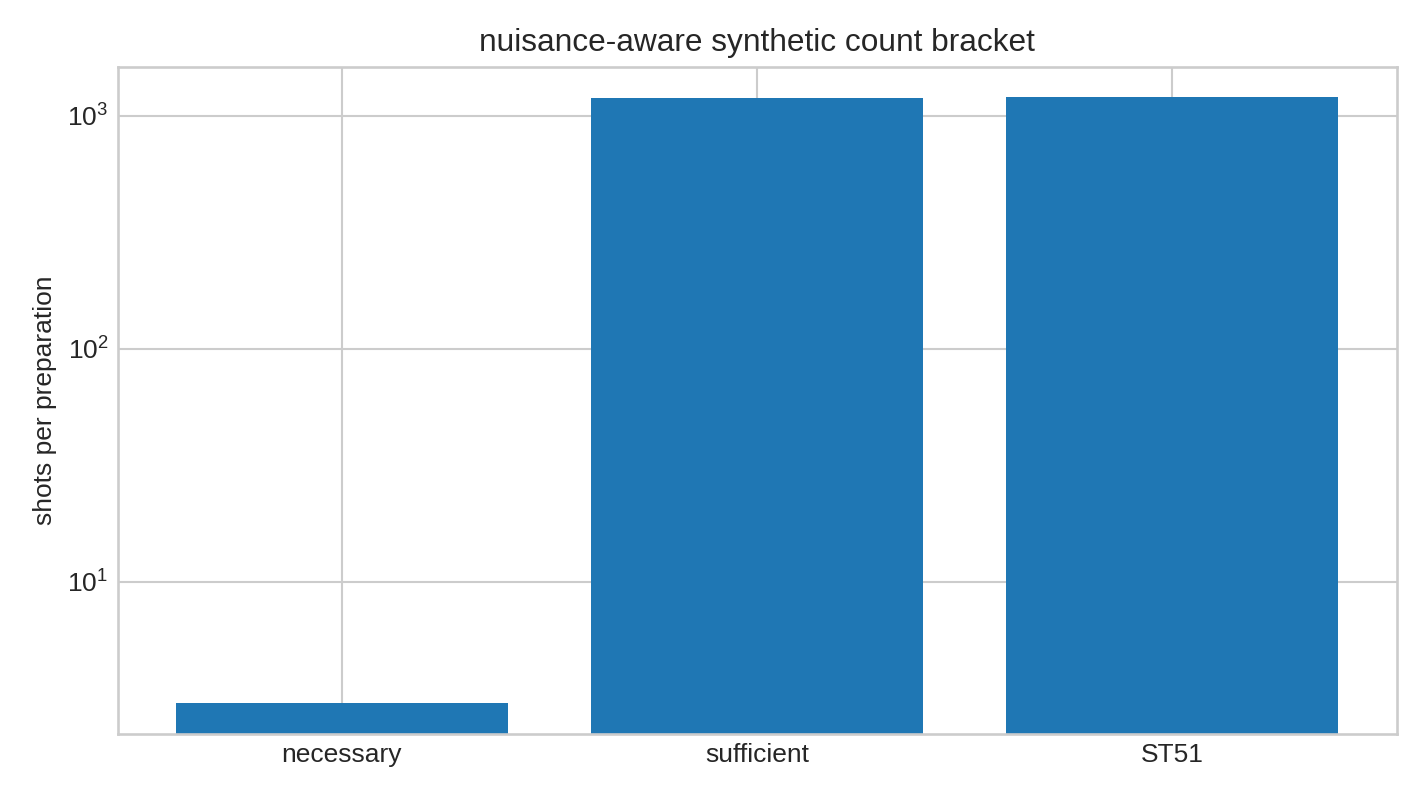
\includegraphics[width=0.70\textwidth]{FIN_ST70_ST81_Figures/st74_robust_counts.png}
\caption{The declared nuisance model widens the useful synthetic bracket dramatically.}
\end{figure}

\statusboundary{} Loss, dark counts, uniform contamination, calibration balls, carriers, preparations, and outcomes remain synthetic assumptions. This is a receiver-design theorem, not apparatus calibration or a laboratory prescription.

\section{ST75 --- The complete CPTP intertwiner cone}

Consider
\[
\mathcal U_t(\rho)=e^{-itA}\rho e^{itA},\qquad
\mathcal D_\tau(\rho)=e^{-\tau\operatorname{ad}_A^2}(\rho),
\]
at $t=\tau=0.61$. On an energy matrix unit $E_{ij}$ their eigenvalues are
\[
e^{-it(\lambda_i-\lambda_j)},\qquad e^{-\tau(\lambda_i-\lambda_j)^2}.
\]
The first has unit modulus. The second has unit modulus only for zero energy gap. Moreover, the largest strict unitary gap phase is $1.4287311<2\pi$, so a unitary eigenvalue can equal $1$ only at zero gap.

Let $\Pi$ be pinching onto equal-energy blocks. Their multiplicities are
\[
(1,2,2,2,2,2,1),
\]
and their algebra has complex dimension
\[
1^2+5\cdot2^2+1^2=22.
\]

\begin{theorem}[Complete finite intertwiner characterization]
A linear map $\Phi$ satisfies $\Phi\circ\mathcal U_t=\mathcal D_\tau\circ\Phi$ if and only if
\[
\Phi=\Pi\circ\Phi\circ\Pi.
\]
The complex intertwiner space therefore has dimension $22^2=484$. Its CPTP cone is exactly
\[
J(\Phi)\succeq0,\qquad \operatorname{tr}_{\rm out}J(\Phi)=I,
\qquad \Phi=\Pi\Phi\Pi.
\]
\end{theorem}

Spectral pinching and Gibbs reset are distinct CPTP examples, with sampled intertwining residuals below $10^{-15}$. This strictly extends the earlier spectral-Schur example.

\begin{figure}[H]
\centering
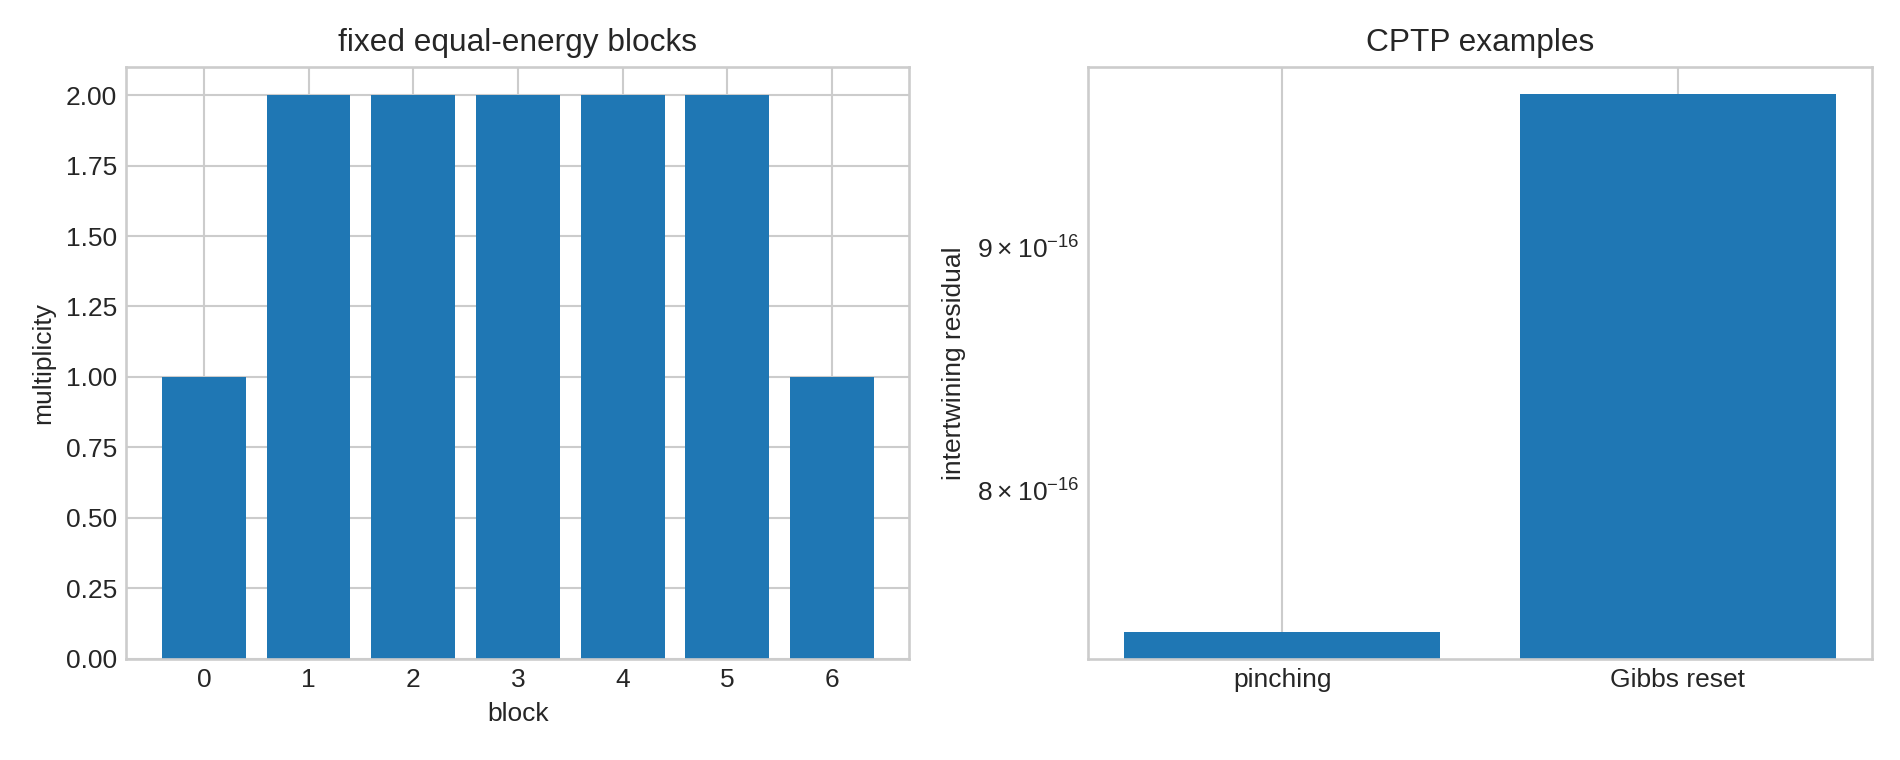
\includegraphics[width=0.92\textwidth]{FIN_ST70_ST81_Figures/st75_cptp_cone.png}
\caption{Equal-energy blocks and two inequivalent CPTP intertwiners.}
\end{figure}

\statusboundary{} The theorem concerns unitary evolution and quantum $A$-dephasing. It neither identifies a physical carrier nor equates either channel with the classical vertex heat semigroup.

\section{ST76 --- Minimal conditional thermodynamic resources}

ST64 supplied the identity after adding thermodynamic structure. ST76 applies removal tests to the target package: dimensionful energy, dimensionful entropy, a Gibbs equilibrium, and operational nonnegative entropy production.

\begin{center}
\small
\begin{tabularx}{0.96\textwidth}{@{}p{0.25\textwidth}X@{}}
\toprule
Removed resource & Countermodel or ambiguity\\
\midrule
Positive energy scale $E_*$ & $A$ and $cA$ have identical dimensionless records after inverse time/temperature rescaling but assign different energy/work\\
Entropy unit $k_*$ & $S_{\rm vN}$ and $cS_{\rm vN}$ are indistinguishable dimensionless information conventions\\
Gibbs reference/bath $\gamma$ & No preferred inverse temperature, equilibrium comparison, or free-energy zero remains\\
$\gamma$-preserving process and heat/work instrument & An arbitrary channel can prepare a higher-resource state from $\gamma$; operational heat is undefined\\
\bottomrule
\end{tabularx}
\end{center}

\begin{theorem}[Relative resource minimality]
The four resource types above are independently necessary and jointly sufficient for the standard relative-entropy/free-energy identity and its data-processing monotonicity, relative to the declared target semantics.
\end{theorem}

\begin{figure}[H]
\centering
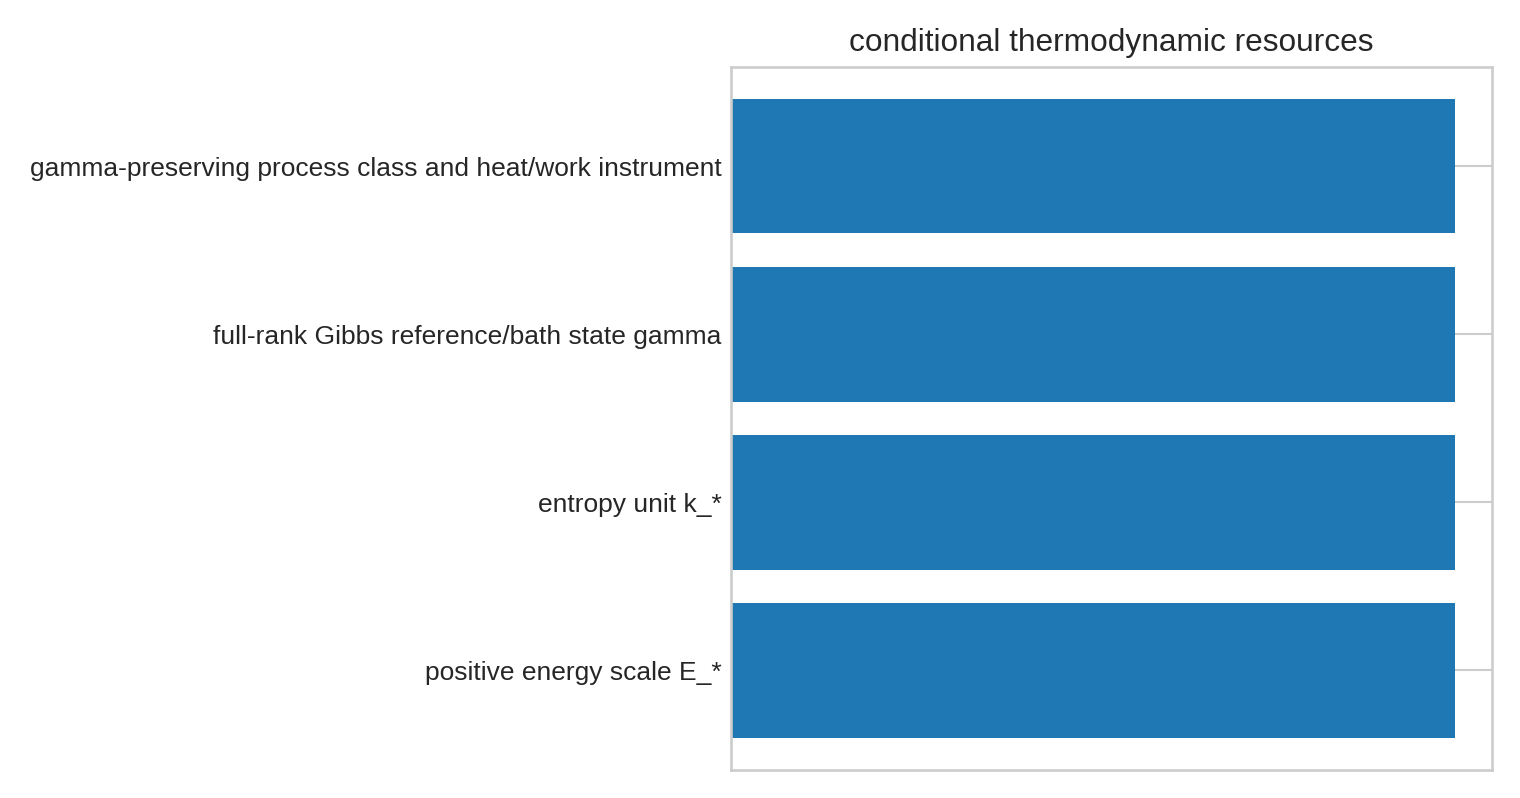
\includegraphics[width=0.78\textwidth]{FIN_ST70_ST81_Figures/st76_resource_minimality.png}
\caption{Four independently necessary types in the conditional thermodynamic package.}
\end{figure}

\statusboundary{} ``Minimal'' is relative to the stated operational target and object types. It does not derive $E_*$, $k_B$, a bath, a temperature, or an experimental instrument from the strict operator.

\section{ST77 --- The localized branch crosses a fold}

The ST65 stationary equation was restricted to the seven-dimensional reflection-fixed subspace and augmented by a pseudo-arclength constraint. A predictor--corrector continuation crosses the loss of invertibility that stopped fixed-$\kappa$ continuation. Solving the augmented fold system
\[
F(u,\kappa)=0,\qquad D_uF(u,\kappa)v=0,\qquad \|v\|^2=1
\]
gives
\begin{align*}
\kappa_{\rm fold}&=0.01658905238638291,\\
\operatorname{IPR}(u_{\rm fold})&=0.9776497495222588,\\
\|G_{\rm fold}\|_\infty&=8.33\times10^{-17}.
\end{align*}
The numerical augmented Jacobian has minimum singular value $0.08025$, supporting a simple fold. Continuation then returns to $\kappa=0.01198$ on the second local sheet.

\begin{figure}[H]
\centering
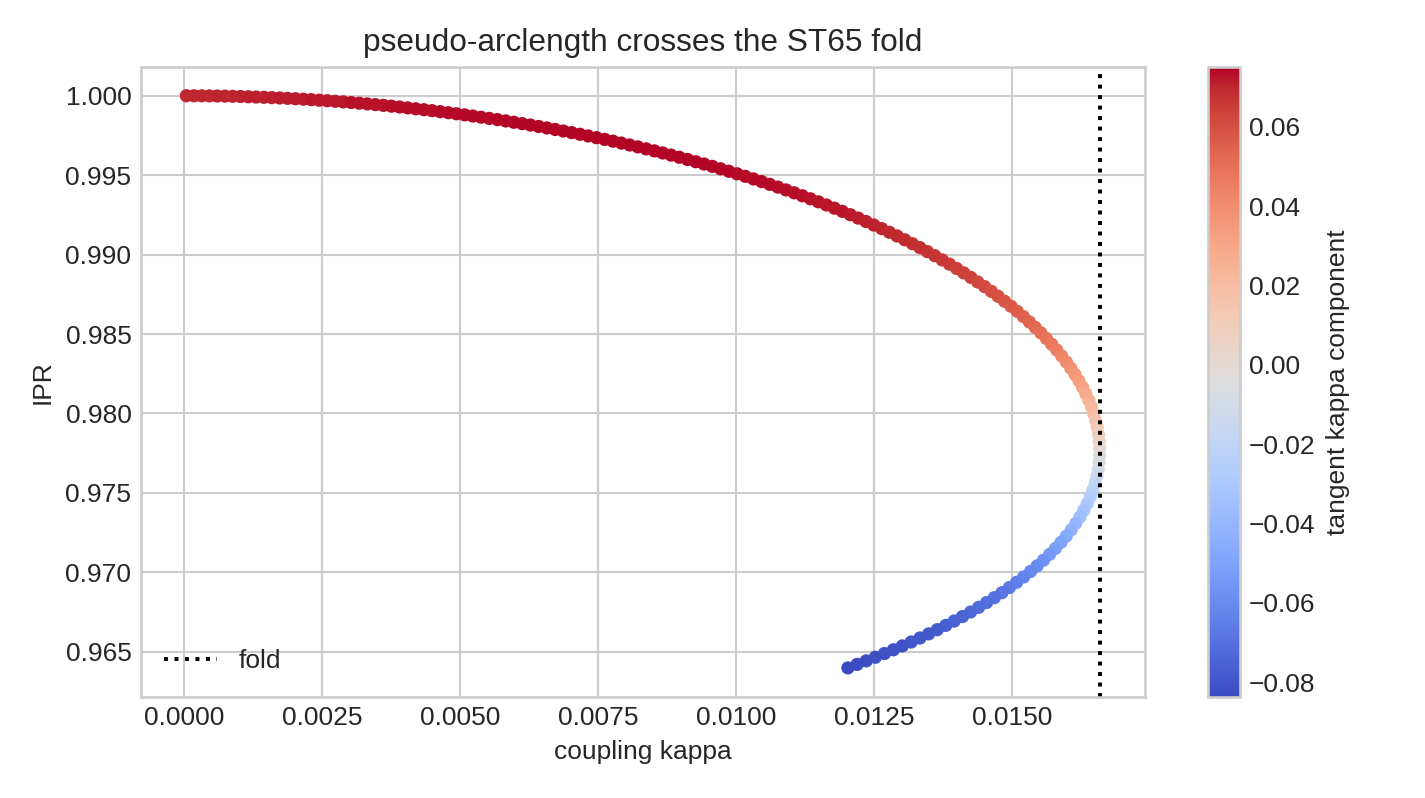
\includegraphics[width=0.76\textwidth]{FIN_ST70_ST81_Figures/st77_pseudo_arclength.png}
\caption{The tangent's $\kappa$ component changes sign at the first fold; the branch returns rather than terminating.}
\end{figure}

\strong{} This is a substantive correction: ST65's fixed-parameter failure was a fold, not evidence that the branch ended. \statusboundary{} The calculation is binary64 numerical continuation. It does not interval-certify the fold, continue to $\kappa=1$, establish stability, or exclude disconnected branches.

\section{ST78 --- Strict-doublet backreaction}

Embedding the ST66 complex order parameter $z$ in the first strict Fourier doublet adds the quadratic stiffness
\[
\frac g2\lambda_1|z|^2,
\qquad \lambda_1=0.754121154207080.
\]
The effective control parameter becomes $\mu_{\rm eff}=\mu-g\lambda_1$. In terms of $y=|z|^2$, the radial equation is
\[
-(\mu-g\lambda_1)+y-0.01y^5+0.01y^6=0.
\]
The remaining function is strictly increasing and nonnegative on $y\ge0$: for $y\le5/6$ its derivative is greater than $1-0.05(5/6)^4>0$, and for $y\ge5/6$ the two high-order derivative terms have nonnegative sum.

\begin{theorem}[Conditional quenching threshold]
There is exactly one positive radial branch for
\[
g<g_c=\mu/\lambda_1=0.4641164062928421,
\]
and none for $g\ge g_c$. Thus the constructed twelve-branch phase is quenched at unit strict coupling.
\end{theorem}

\begin{figure}[H]
\centering
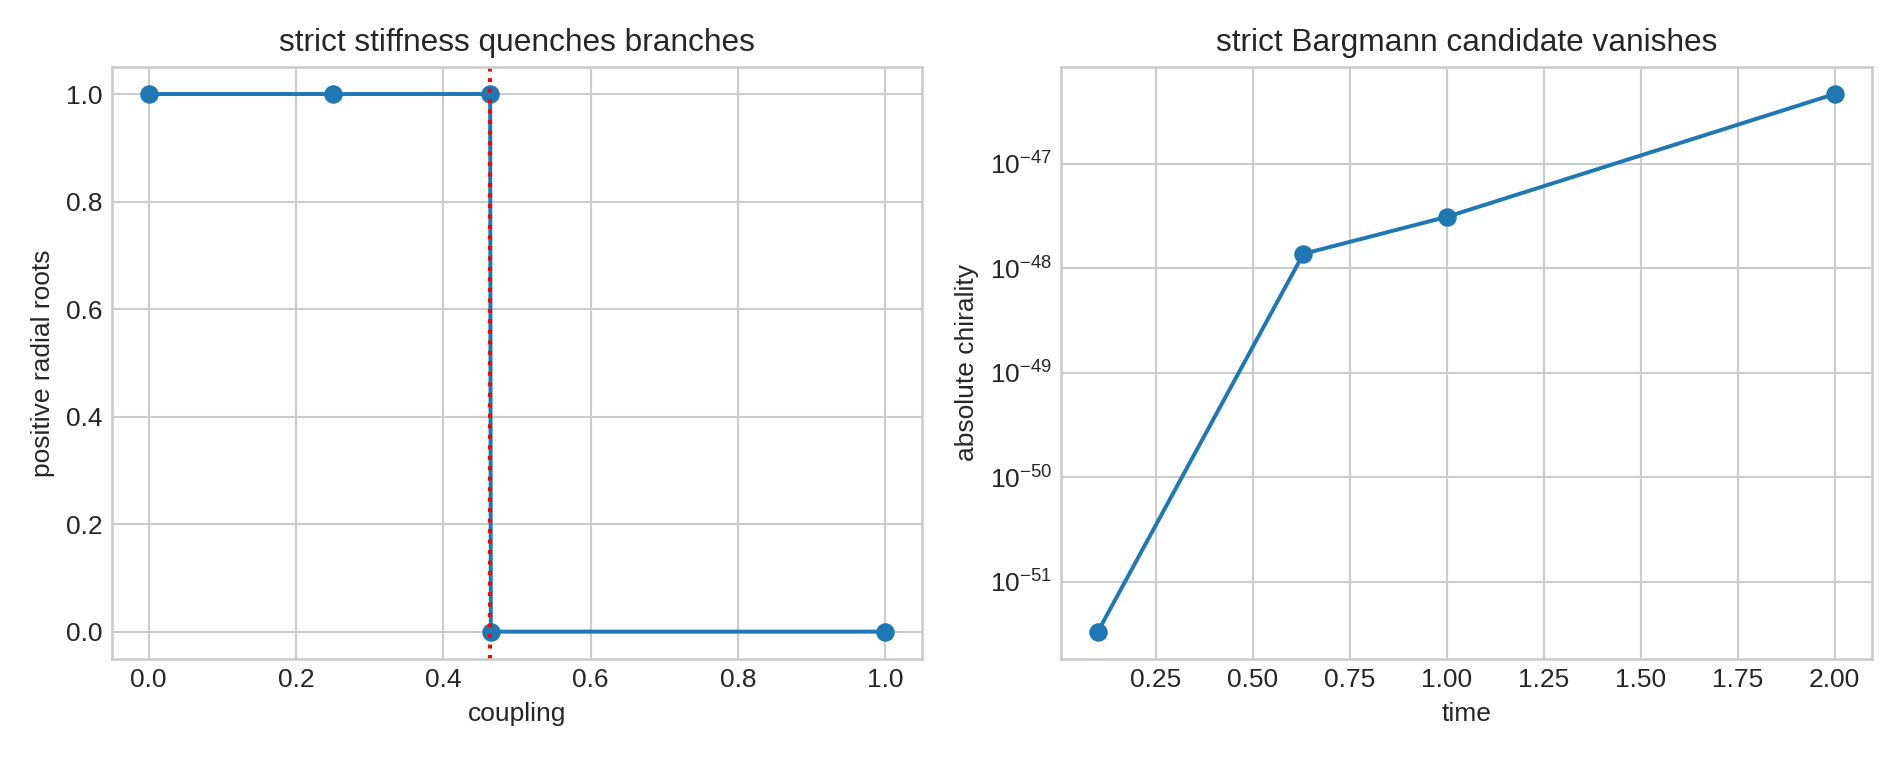
\includegraphics[width=0.93\textwidth]{FIN_ST70_ST81_Figures/st78_backreaction_st79_chirality.png}
\caption{Conditional strict stiffness removes the constructed radial branches; strict functional-calculus chirality remains zero.}
\end{figure}

\statusboundary{} The result falsifies the naive assumption that adding strict stiffness preserves the ST66 phase. The potential, coupling, and identification of $z$ remain inserted; it is not a no-soliton theorem for other nonlinear laws.

\section{ST79 --- Stabilizer obstruction to strict chirality}

Let $R$ be reflection. Since $RAR^{-1}=A$, every deterministic stabilizer-covariant ray assignment $\mathcal R(A)$ must be reflection invariant. The gauge-invariant summed imaginary Bargmann product
\[
\chi(\mathcal R)=\sum_x\operatorname{Im}
\bigl(\langle r_x,r_{x+1}\rangle
\langle r_{x+1},r_{x+2}\rangle
\langle r_{x+2},r_x\rangle\bigr)
\]
is reflection odd.

\begin{theorem}[Strict stabilizer no-go]
Every deterministic stabilizer-covariant Bargmann chirality sourced only by scalar strict $A$ vanishes: $\chi(A)=0$.
\end{theorem}

Indeed $\chi(A)=\chi(RAR^{-1})=-\chi(A)$. Rows of $e^{-itA}$ at four times give absolute values below $4.7\times10^{-47}$, a numerical shadow of the exact symmetry result.

\statusboundary{} Orbit-valued assignments, projective lifts, state histories, boundaries, or records can evade the theorem only by supplying the missing symmetry-breaking data. This is not QW-2191 closure.

\section{ST80 --- Signed custody validation}

The executable packet now includes:
\begin{itemize}
\item a hash of the raw event list and a separate hash of frozen nuisance bounds;
\item four pairwise-distinct Ed25519 public keys;
\item a hash-linked provider $\to$ registrar $\to$ analyst $\to$ custodian attestation chain;
\item signature verification against packet public keys;
\item frozen holdout, one pipeline run, and no-refit-after-failure flags.
\end{itemize}
The valid synthetic packet is accepted. A one-event alteration and a duplicated public key are rejected.

\begin{figure}[H]
\centering
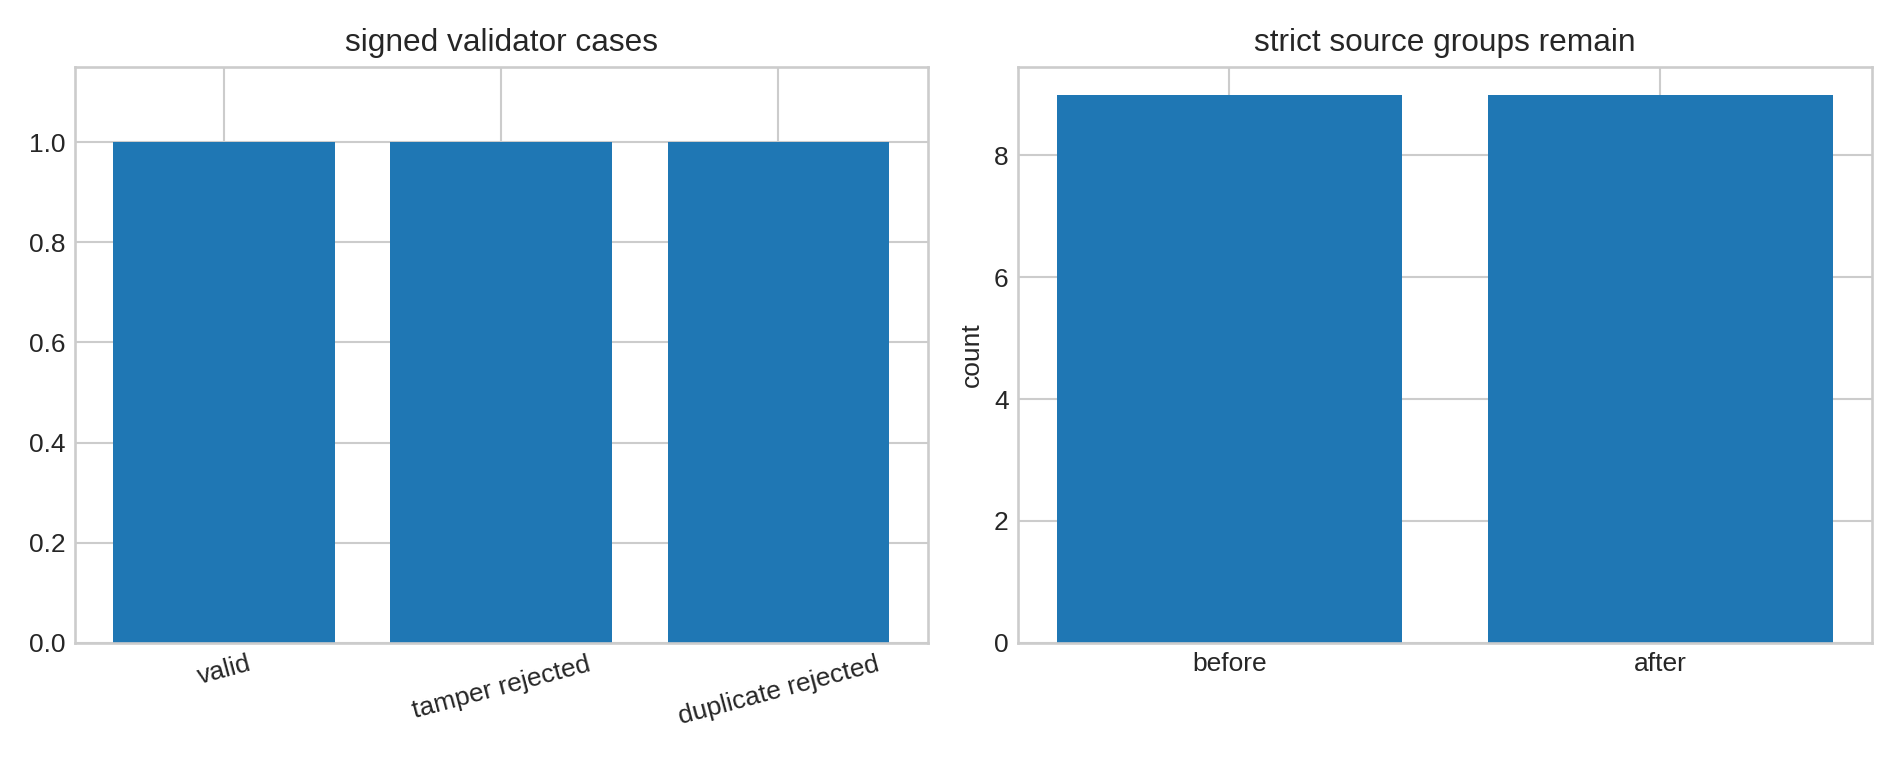
\includegraphics[width=0.92\textwidth]{FIN_ST70_ST81_Figures/st80_validator_st81_sources.png}
\caption{The validator rejects declared integrity failures; the strict source count does not change.}
\end{figure}

\constructed{} The signatures prove possession of the corresponding test private keys and integrity of signed bytes. \statusboundary{} All four deterministic keys and all events were generated locally. They do not establish human identity, organizational independence, trustworthy calibration, or laboratory custody.

\section{ST81 --- W0+CA+SA architecture after falsification}

The nine source groups can be made more legible without pretending they have disappeared:
\begin{center}
\small
\begin{tabularx}{0.96\textwidth}{@{}p{0.12\textwidth}p{0.25\textwidth}X@{}}
\toprule
Package & Contents & Current boundary\\
\midrule
W0 & strict dimensionless operator and certified consequences & Proven core; operator provenance and physical role remain separate\\
CA & energy, entropy, time/length conversion resources & ST76 proves conditional necessity, not strict derivation\\
SA & state, orientation, gain, projective/spin, memory realization & ST71/72/79 expose missing one-sided and lift data\\
RA & refinement and fine-data code & ST73 is unique only after a record and penalty are supplied\\
OA & preparation, channel, instrument, calibration, record, custody & ST75/80 construct mathematics and syntax, not a laboratory\\
\bottomrule
\end{tabularx}
\end{center}

\begin{theorem}[No source-group reduction]
ST70--ST80 strengthen proof replay and conditional completion packages, but every proposed gain, spin, refinement, thermodynamic, nonlinear, chirality, and custody mechanism retains at least one added typed source. All nine strict physical-source groups therefore remain relative to the declared targets.
\end{theorem}

The ontology guardrail is unchanged: the nadsoliton is the primordial fractal information in a solitonic state, with no lower informational layer. The internal intended order remains nadsoliton $\to$ light $\to$ matter $\to$ emergent observer. These ontological statements do not alter the proof statuses above.

\section{Falsification ledger}

\begin{itemize}
\item \textbf{Independent replay did not become full rederivation.} ST70 passed every exact exported inequality but preserved the transcendental trust boundary.
\item \textbf{Positive gain became a one-sided axiom target.} ST71 proves precisely which order condition is required; it does not find its source.
\item \textbf{Spin availability separated from spin selection.} ST72 proves $C_{24}$ exists and proves scalar blindness to the choice.
\item \textbf{Fine data solve and relocate refinement nonuniqueness.} ST73 makes $q$ unique only by adding a record and rate penalty.
\item \textbf{Ideal count optimism was destroyed.} ST74's conservative robust sufficient mean, 1,192, is near the old synthetic 1,200 setting rather than ST62's ideal five.
\item \textbf{The CP picture enlarged but remained irreversible.} ST75 finds an entire cone, not an invertible physical equivalence.
\item \textbf{Thermodynamics was not generated by entropy notation.} ST76 isolates four independently necessary resource types.
\item \textbf{The ST65 interpretation was falsified.} The branch folds and returns; it was not numerically terminated.
\item \textbf{Naive backreaction persistence was falsified.} Unit strict stiffness quenches the constructed ST66 branches.
\item \textbf{Strict scalar chirality was obstructed.} Reflection forces every deterministic stabilizer-covariant Bargmann scalar to zero.
\item \textbf{Cryptographic syntax remained operationally incomplete.} Local test signatures cannot create independent custody.
\end{itemize}

The deepest surviving interpretation is a \emph{finite spectral-information core with exact quotient, symmetry, and operator-channel theorems, plus a nonunique typed completion layer}. Mathematical strengthening repeatedly identifies the missing source more sharply; it has not made the source disappear.

\section{Recommended programs ST82--ST93}

\small
\begin{longtable}{@{}p{0.08\textwidth}p{0.10\textwidth}p{0.74\textwidth}@{}}
\toprule
Program & Priority & Research test\\
\midrule
\endfirsthead
\toprule
Program & Priority & Research test\\
\midrule
\endhead
ST82 & 1 & Independently regenerate every ST58 transcendental and matrix enclosure with Arb/Sage or a proof assistant.\\
ST83 & 2 & Interval-certify the ST77 simple fold and its local return branch in the seven-variable reflection sector.\\
ST84 & 3 & Seek a strict temporal-order source in admissible memory realizations, or prove a passivity/detailed-balance obstruction.\\
ST85 & 4 & Classify state- or boundary-sourced lifts to $C_{24}$ without silent selector insertion.\\
ST86 & 5 & Derive a fine-record statistic from an explicit local compression/RG map and test refinement universality.\\
ST87 & 6 & Replace ST74's conservative concentration bound by a robust likelihood convex dual and exact nuisance optimization.\\
ST88 & 7 & Classify extreme points and reversible faces of the ST75 CPTP intertwiner cone.\\
ST89 & 8 & Formalize ST76 resource independence and distinguish thermal operations from Gibbs-preserving maps.\\
ST90 & 9 & Continue the ST77 branch beyond its first return and run a symmetry-classified disconnected-branch search.\\
ST91 & 10 & Analyze dynamic strict-doublet/order-parameter backreaction and stability across the ST78 threshold.\\
ST92 & 11 & Search for one genuinely strict-sourced reflection-odd object outside scalar functional calculus.\\
ST93 & 12 & Export a machine-readable W0+CA+SA+RA+OA theory schema with claim-level dependency proofs.\\
\bottomrule
\end{longtable}
\normalsize

The highest proof-value tasks are ST82 and ST83. The highest conceptual tasks are ST84--ST86: time orientation, the spin lift, and fine-data refinement are now sharply typed rather than vaguely ``missing.''

\section{Reproducibility}

The release contains the deterministic source, twenty-four live tests, complete JSON/CSV results, the ST70 rational replay, ST74 count packet, ST80 signed validator, eight figures, input hashes, and a release manifest. The local replay is
\[
\texttt{MPLCONFIGDIR=/tmp/fin-st70-mpl python3 fin\_st70\_st81\_research.py}
\]
followed by
\[
\texttt{MPLCONFIGDIR=/tmp/fin-st70-mpl python3 -m unittest -v test\_fin\_st70\_st81.py}.
\]
All 24 tests passed. No network, laboratory data, or external service is needed. This reproducibility statement covers local mathematics and synthetic protocols only.

\section{Final conclusion}

ST70--ST81 close several finite mathematical questions and correct one important numerical interpretation:
\begin{enumerate}
\item the exported ST58 bracket passes an independent exact-rational acceptance replay;
\item positive gain is equivalent to an explicitly one-sided response cone, not to symmetry alone;
\item a nontrivial $C_{24}$ spin cover exists, but strict scalar data do not choose it;
\item fine records can select refinement, while coarse strict $A$ cannot supply those records;
\item robust nuisance assumptions widen the synthetic count bracket from ideal units to thousands of total events;
\item the complete CPTP intertwiner family factors through a 22-dimensional block algebra and occupies a 484-dimensional linear space;
\item four thermodynamic resource types are relatively independently necessary;
\item the localized branch encounters a simple numerical fold and returns rather than terminating;
\item unit strict stiffness quenches the constructed ST66 phase above $g_c\simeq0.4641$;
\item reflection obstructs deterministic strict-sourced Bargmann chirality;
\item signed local packets improve integrity syntax but do not create real custody;
\item all nine strict physical-source groups remain.
\end{enumerate}

No QW-2191 discharge, strict time/gain/spin/refinement/dimensional source, laboratory evidence, legacy-to-strict completion, legacy-role transfer, Standard Model, gravity, $L_{\rm total}$, or Theory-of-Everything closure is exported.

\vfill
\begin{center}
\small Release 10.60 --- English research report --- CC BY 4.0
\end{center}

\end{document}
